In this chapter background research conducted into similar applications, and concepts will be investigated. 
\section{Weasley Clock}

The project undertaken was proposed as the creation of a Weasley digital clock. The Weasley clock is a magical clock owned by the Weasley family in the famous Harry Potter series. The hours were replaced by locations such as Home, and Mortal Peril which would represent the potential status of each family member. Each family member had a clock hand that would point to their status at any point in time. This project's goal was to make a digital version of this Weasley clock. 
\begin{figure}[!htbp]
    \centering
    \begin{subfigure}[b]{0.25\textwidth}
        \frame{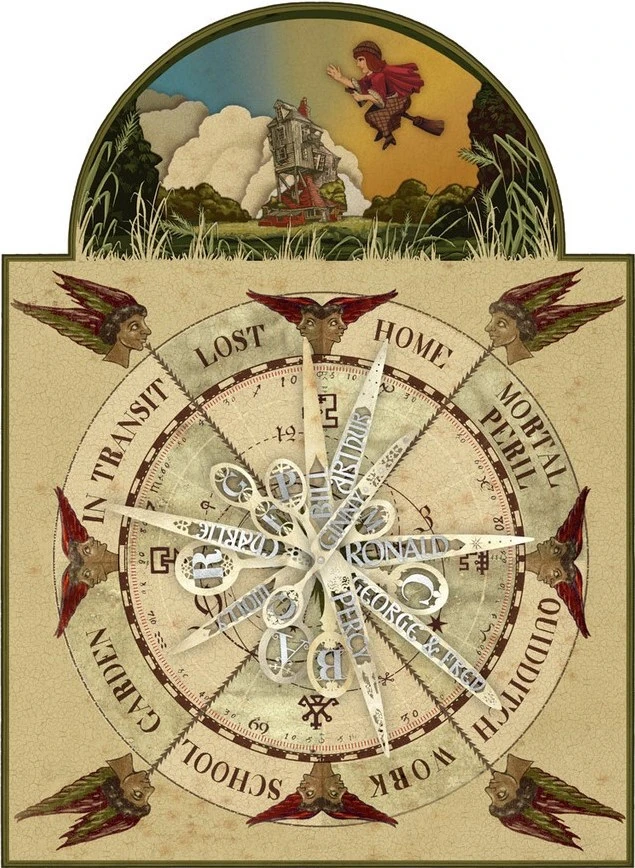
\includegraphics[width=\textwidth]{The_Weasley_Family_Clock.png}}
    \end{subfigure}
    \caption[The Weasley clock]{The Weasley clock \cite{weasClockWiki}}
    \label{fig:weasClock}
\end{figure}
\FloatBarrier

\section{Existing Applications}
Similar concepts and existing applications were investigated, and evaluated before the project began. These are discussed below. 


\subsection{Snapchat Maps}
Snapchat is a leading social media application widely used throughout the world. Snapchat maps is an application feature that when enabled broadcasts a user's location on a map for all their friends to see. In a research article by Rowan Wilken and Lee Humphreys \cite{snapMaps}, it was discussed how although at first the concept of displaying a user's location received negative responses, attitudes shifted and now this feature has shown positive societal uses, such as when Snapchat maps were used to help rescue hurricane victims who were broadcasting their locations. This feature shows with its popularity how users like to be able to see where their friends are, and what they are doing at any point in time through a graphical representation. 

\begin{figure}[!htbp]
    \centering
    \begin{subfigure}[b]{0.6\textwidth}
        \frame{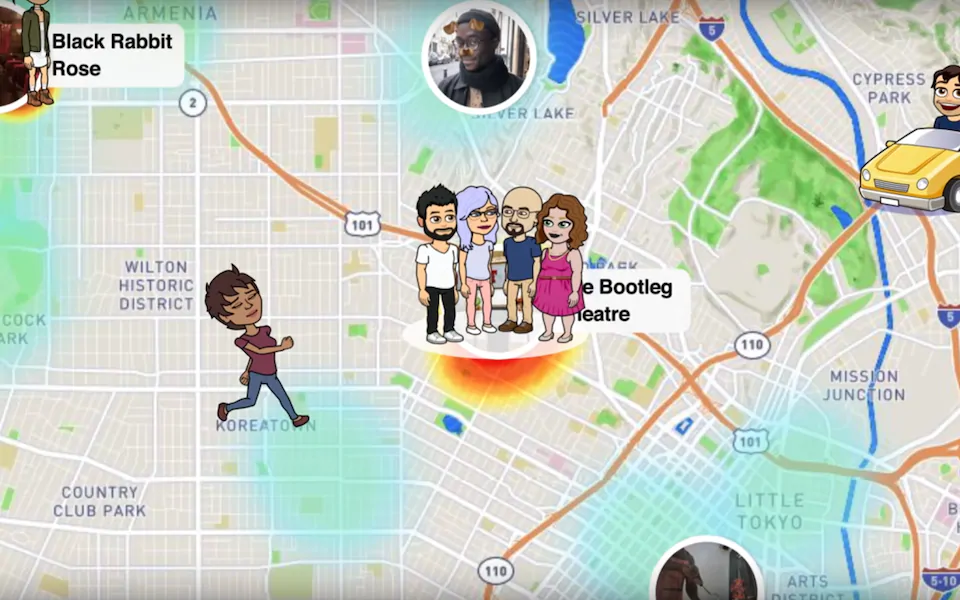
\includegraphics[width=\textwidth]{snapMap.png}}
    \end{subfigure}
    \caption[Snapchat Maps]{Snapchat Maps \cite{snapMapImg}}
    \label{fig:snapMap}
\end{figure}
\FloatBarrier

Although this application differs from the project proposal, some ideas, and features were transferable. The idea of groups of friends being able to view a graphical representation of their friend's status is a key goal of this project with the difference being that a user's location is displayed on a clock. Users can add friends and create groups which is another feature that would be implemented during the project. However, there are features that Snapchat maps lack that would be good to implement in this project such as customisation of profiles, adding to the user experience.

\subsection{Life360}

Life360 is a location sharing social media application that was created in 2008 but has risen to high popularity over the last few years. Life360 was designed as a `family social network' which would allow a family to create a \textit{circle} to which they would use the application with. However, this application has become more than this, groups of friends have now utilised this application, creating their own circles to use the application. The application was studied by Hasinoff \cite{life360}, where it was discussed how the application sells a service that collects, repackages, and then presents the user's personal data. This study examines how the application is used and marketed to give users a feeling of safety from the use of the application, but there are pitfalls. The app has many features such as `Location Safety', where you can view your journeys, places you have visited, and see other circle members' location data. The app also has an array of `Driving Safety' features, but these are not related to this project. 

\begin{figure}[!htbp]
    \centering
    \begin{subfigure}[b]{0.21\textwidth}
        {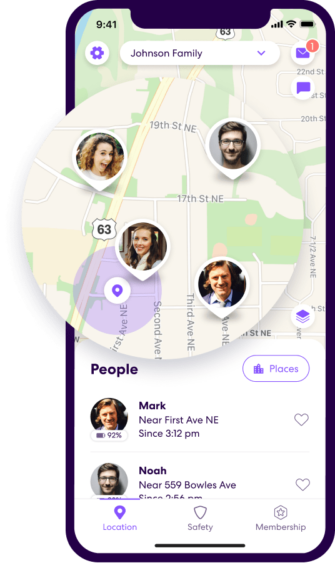
\includegraphics[width=\textwidth]{life360.png}}
    \end{subfigure}
    \caption[Life360]{Life360 \cite{lifeLoc}}
    \label{fig:life360}
\end{figure}
\FloatBarrier

Some features, and concepts from this app can be transferred to this project. The ability for users to create their own `circles' with peers, the concept of users wanting to know their friend's status, and the ability to view their friend's status graphically without having to ask are all concepts that could also be used in this project. However, there are many areas of Life360 that are not appropriate or useful for this application. The push for constant data sharing, hiding helpful features behind a paywall, and the controlling nature of the application are a few disadvantages. This project will improve upon this by simplifying the representation of group members' statuses, removing the privacy issues and controlling nature of the application, and making a more friendly, and simpler design concept. 

\subsection{Magic Clock}

An application that was noted in this project's proposal was Magic Clock \cite{magicClock}. Magic Clock was a project completed by four Media Informatics students at the University of Munich. This Magic Clock project is built upon the same concept as the project being undertaken, where a group of friends has hands on a clock face pointing to their current status. However, the Magic Clock project combined both a hardware, and software implementation of the clock, with the former being controlled by the latter. As the project being discussed in this dissertation is a mobile application, there are several differences between the two projects, but the underlying concept is the same. 

\begin{figure}[!htbp]
    \centering
    \begin{subfigure}[b]{0.22\textwidth}
        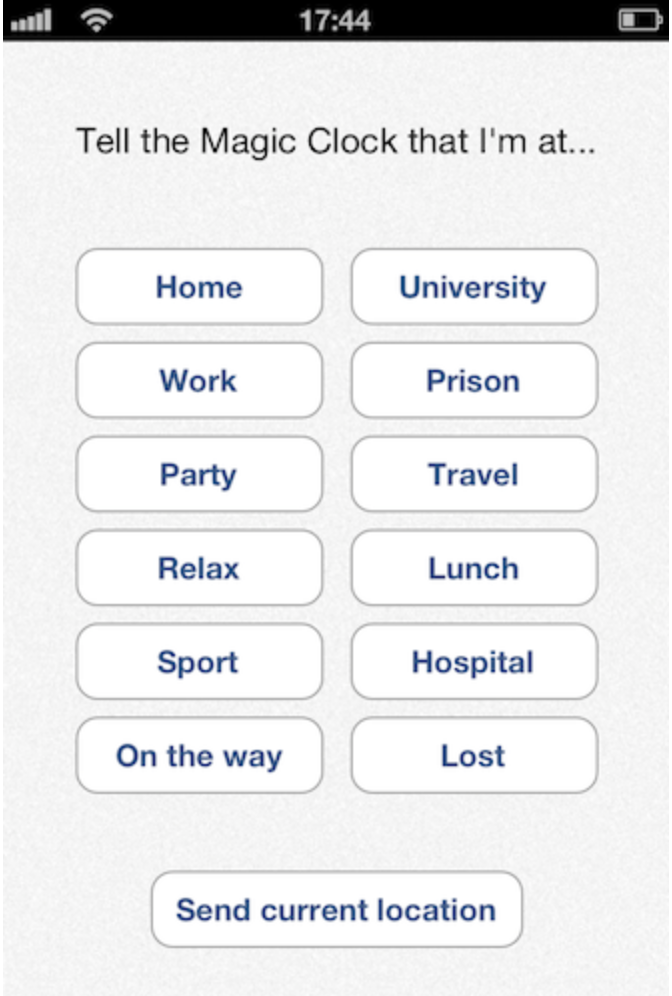
\includegraphics[width=\textwidth]{magClock.png}
    \end{subfigure}
    \hspace{1.5em}
    \begin{subfigure}[b]{0.22\textwidth}
        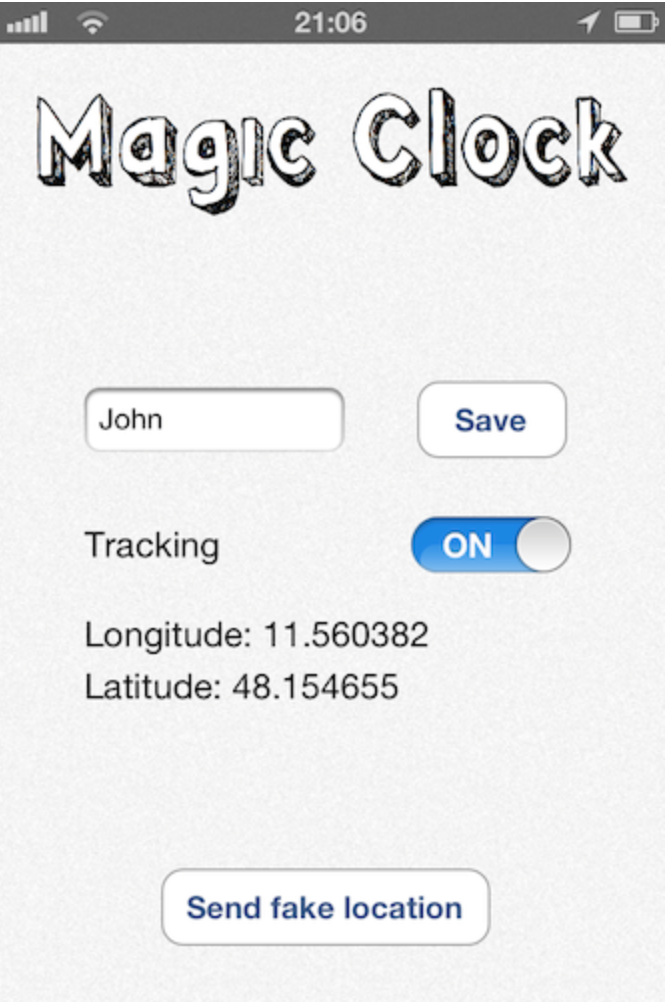
\includegraphics[width=\textwidth]{magClock1.png}
    \end{subfigure}
    \hspace{1.5em}
    \begin{subfigure}[b]{0.22\textwidth}
        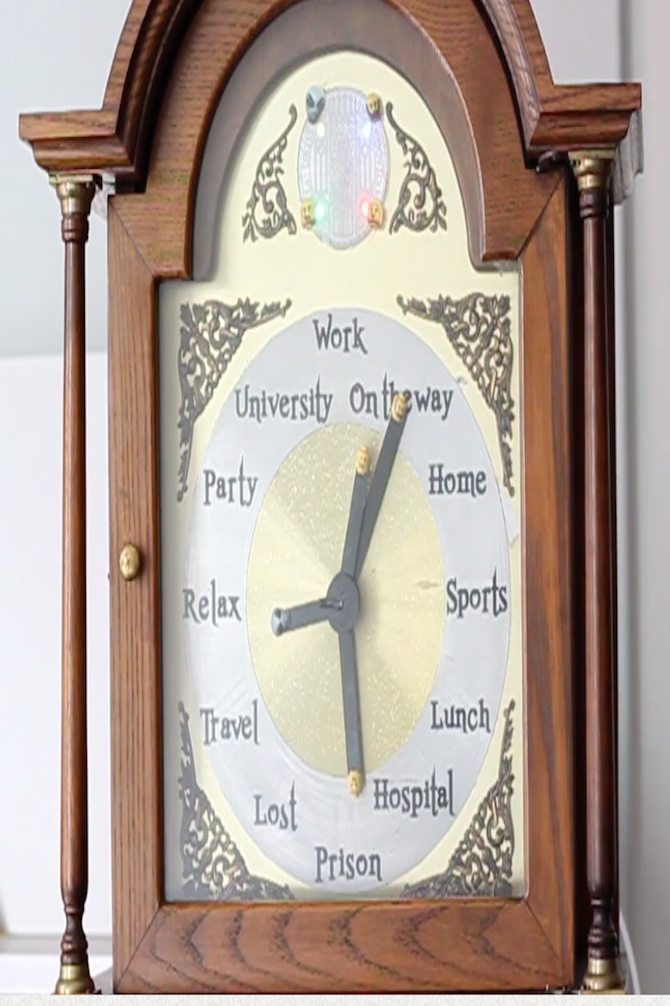
\includegraphics[width=\textwidth]{magClock3.png}
    \end{subfigure}
    \caption{Magic Clock}
    \label{fig:magClock}
\end{figure}
\FloatBarrier

This project aims to create a mobile application of this concept that will be more usable, and more aesthetically pleasing, as the design of the application above could be vastly improved. This application will allow the creation of multiple groups, instead of a sole group in Magic Clock due to not requiring a physical implementation. This project will improve upon Magic Clock by allowing groups of friends to have multiple groups, having a more usable, and aesthetically pleasing user interface, and allowing users to have a mobile implementation of the concept.

\subsection{Microsoft Whereabouts Clock}

In 2006 employees of Microsoft published a research article, the Whereabouts Clock \cite{micrWher}, discussing the early research of a situated awareness device. The idea was to provide users with a way to socially connect by using mobile devices to share their location. Previous work from Sellen et al. \cite{sellen} shared that parents place high importance on knowing their family members' statuses for planning events, and social communication, this was a key motivation for this research. This research shown positive results with further research by Sellen published again in 2009 \cite{sellen2009}. This implementation was similar to the Weasley clock with a user's icon placed in a sector, displaying their status, and an inner circle for users whose status was different from the presets. The results shown that the awareness of other users' statuses from the clock was supporting communication, coordination, and connectedness within groups of users. It was also shown during a trial that households made good use of the prototype developed and reacted positively with great interest shown for the concept.

\begin{figure}[!htbp]
    \centering
    \begin{subfigure}[b]{0.5\textwidth}
        {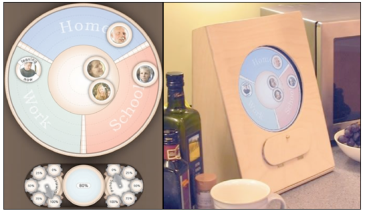
\includegraphics[width=\textwidth]{MicroWhere.png}}
    \end{subfigure}
    \caption{Microsoft Whereabouts Clock}
    \label{fig:microWhere}
\end{figure}
\FloatBarrier

This research from Microsoft confirmed that there was a market for such a product and that people were interested. However, there are some areas that the Weasley clock application could improve upon this idea. By making the clock part of a mobile application, there would likely be more user interaction due to humans predominantly choosing software solutions over hardware in this digital age. This would also allow users to have multiple groups where they could gain these social benefits uncovered through this research. This project will also improve upon the design of the clock as although this was designed in 2009, the design could be vastly improved upon. 



\section{Summary}

In summary, there were an array of existing concepts, and applications researched to provide a basis for this project. Although undoubtedly some of these products have had great successes, there are areas in which they can be improved. This background research helped develop a greater understanding of the project, providing ideas that can be built upon and improved in this application.